\subsection{Map}
The map shows the status of the countries on Earth at this certain moment of history set in the timeline -- the \textbf{NowDate}. For this project we used a self-made dataset of historic countries of whole Europe from 1945 until today and from Western, Northern, Southern and Central Europe from 1871 until 1945. We organized the data in a way that we can visualize historic changes of countries on the map. Finally we provided a functionality to style the areas due to a current theme, for example all countries belonging to NATO at the NowDate get a blue background color.

\subsubsection{Historic Countries} % (fold)
\label{ssub:historic_countries}

A country consists of an \textbf{area}, represented as a multipolygon geometry and a \textbf{label} with the name of the country and the position of the label.

\paragraph{Areas}
Everything is based on a dataset of the current countries in Europe from \textit{Natural Earth Data}
\footnote{1:10m Cultural Vectors | \url{http://www.naturalearthdata.com/downloads/10m-cultural-vectors/}}.
We extracted only the countries of Europe and loaded them into \textit{QuantumGIS}, an open source GIS software for organizing, analyzing and visualizing areas on Earth. For each historic country we found an historic map online and created the area of the country using the \textit{Vector Geoprocessing Tools} of QuantumGIS. Each area is stored in a single ~ \texttt{area\_id.geojson} ~ file.

\begin{figure}[H]
  \begin{center}
    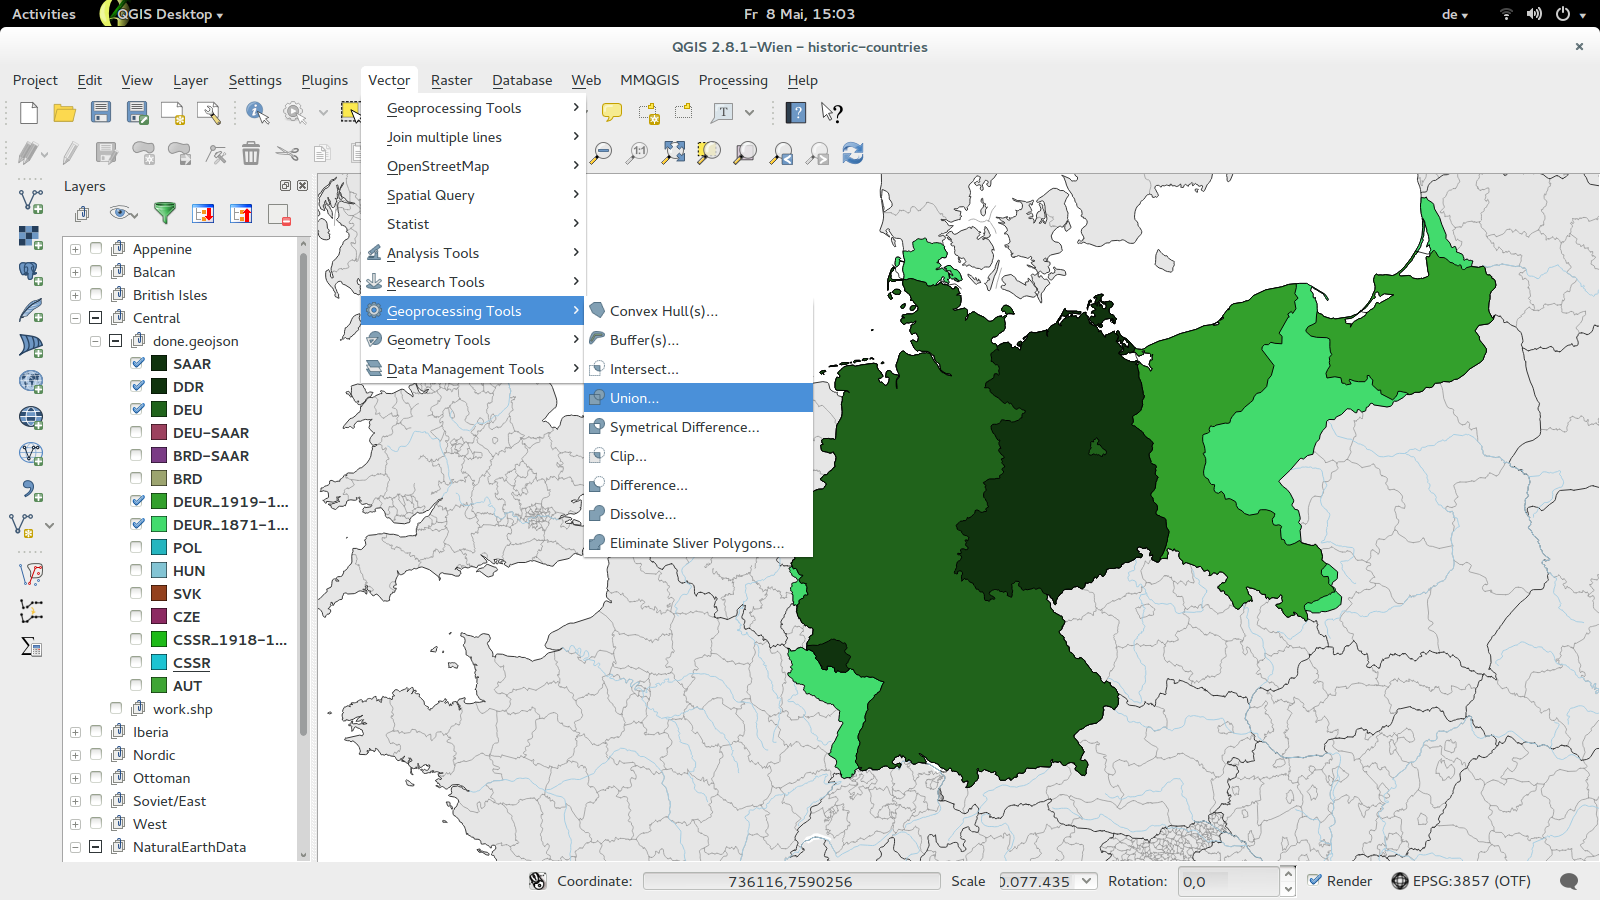
\includegraphics[width=0.9\textwidth]{graphics/qgis.png}
  \end{center}
  \caption{Geometry Manipulation of Historic Countries in QuantumGIS}
  \label{fig:qgis}
\end{figure}
\label{par:area}

In \ref{fig:qgis} you can see the areas of Germany from 1871 until today, from light green to dark green:

\begin{itemize}
  \item 1871 - 1919 German Empire
  \item 1919 - 1945 Weimar Republic and Third German Reich (after WW I)
  \item 1945 - 1949 Occupied Germany (after WW II)
  \item 1949 - 1990 GDR without West Berlin and \\
        1949 - 1956 Saarland
\end{itemize}

Because of the very problematic Usability of QuantumGIS and the mass of data that would have needed to be processed we have not reached the goal to create a data base of all historic countries in Europe from 1871 on, but only from 1945 on, due to the time constraint.

\paragraph{Labels} % (fold)
\label{par:labels}

of a country are set in an table consiting of the id, the label name, the label position and a priority of a label. Labels are stored separately from the areas to account for independent changes of names and geometries: A country can be renamed and borders can change, but both events do not need to correlate. The list of labels is stored in a table ~ \texttt{labels.csv}.

The problem with this approach is that the label position and priority can not be deducted from the area. Therefore, both have to be set by hand. We are aware that this manual approach is not optimal, but for the scope of that project it is suitable. For the future, a data model should be found in which areas and labels are connected but can still change separately from each other.

% paragraph labels (end)

% subsubsection historic_countries (end)

\subsubsection{Historic Changes} % (fold)
\label{ssub:historic_changes}
Because of the way areas and labels are organized, an historic change can easily be modelled:

\begin{table}[H]
\begin{small}
  \caption{Examples of Historic Changes}
  \label{tab:tablename}
  \begin{center}
    \begin{tabular}{lllllll}
    \hline

    \hline
    \textbf{date} & \textbf{name of change} & \\
    \textbf{domain} & \textbf{old} & \textbf{new} \\
    \hline
    25.12.1991 & Dissolution of Soviet Union & \\
    \textit{area:} & CCCP & \pbox{5cm}{EST, LVA, LTU, BLR, \\ UKR, MDA, RUS} \\
    \textit{label:} & CCCP & \pbox{5cm}{EST, LVA, LTU, BLR, \\ UKR, MDA, RUS }\\
    \hline
    03.10.1990 & German reunification & \\
    \textit{area:} & BRD, DDR & DEU \\
    \textit{label:} & BRD, DDR & DEU \\
    \hline
    01.01.1990 & End of Socialistic Republics & \\
    \textit{area:} & & \\
    \textit{label:} & PR-ROU, PR-BGR, PR-HUN, PR-POL & ROU, BGR, HUN, POL \\
    \hline
    01.01.1979 & Separation of Greenland & \\
    \textit{area:} & DNK-with-GRL & DNK, GRL \\
    \textit{label:} & & GRL \\
    \hline
    01.01.1881 & Init state & \\
    \textit{area:} & & DEU-REICH-1871, POL-1871, ... \\
    \textit{label:} & & DEU-REICH-1871, POL-1871, ... \\
    \hline

    \hline
    \end{tabular}
  \end{center}
\end{small}
\end{table}

This event-based data model is maintaines like this: if an historic change appears, it needs to have a date of change, a description of what happened, a set of areas that stop exist and a set that starts to exist from this date in history on -- the same for the labels. Afterwards, the new areas have to be created in \textit{QuantumGIS}, which is most of the work, and new labels have to be defined in the table.

For the future, an editor for storing, managing and analyzing historic changes would be desireable, because the data aqcuisiton part took a large share of the projects time.

In order to visualize the data on the client side, the areas, labels and changes have to be preprocessed on the server. Especially the transition areas and borders have to be generated.

\paragraph{Transitions} are the geometric changes in a change event. There is either a transition area, which is the area that changes the membership of a country (e.g. Alsace-Lorraine 1919 from the German Empire to France) or a transition border, that splits two countries (e.g. The border between Czech and Slovak Republic after the dissolution of Czechoslowakia in 1991). These transitions shall be emphasized with an animation in the moment of the historic change so that it is clearly visible to the user what is currently happening. The transitions are generated like this: For each historic change the set of old and new areas are compared to each other and passes the following decision tree:

% Set the overall layout of the tree
\tikzstyle{level 1}=[level distance=2cm, sibling distance=6cm]
\tikzstyle{level 2}=[level distance=2cm, sibling distance=3cm]
\tikzstyle{level 3}=[level distance=2cm, sibling distance=3cm]

% Define styles for bags and leafs
\tikzstyle{bag} = [text width=3.5cm, text centered]

% The sloped option gives rotated edge labels. Personally
% I find sloped labels a bit difficult to read. Remove the sloped options
% to get horizontal labels.
\begin{center}
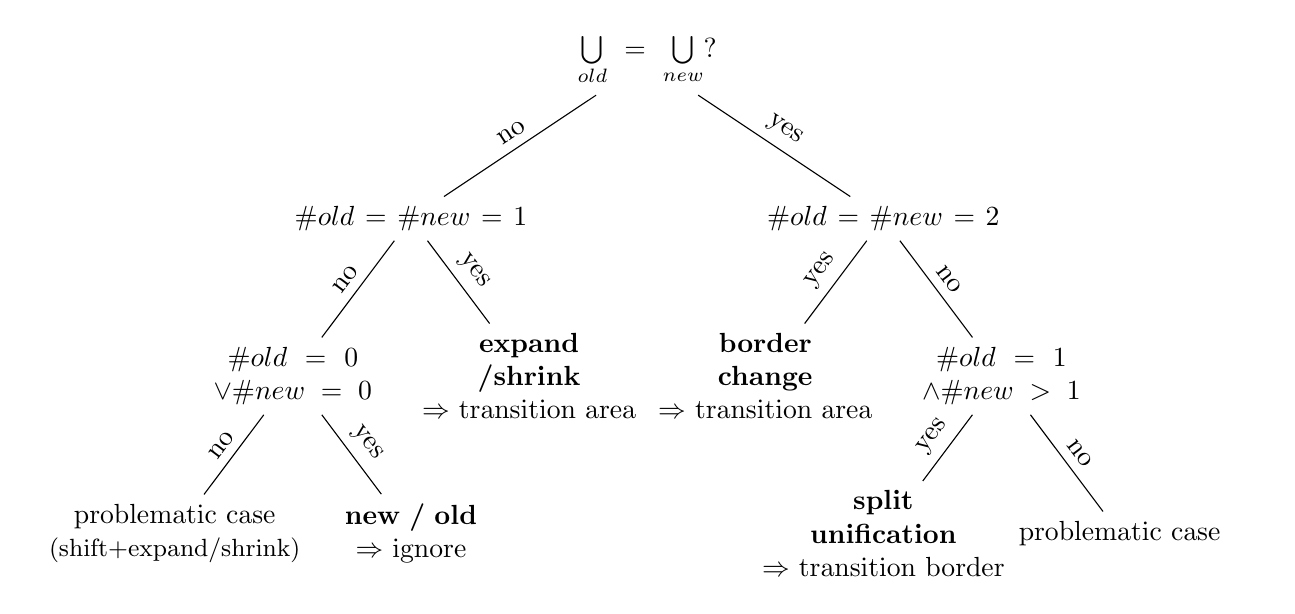
\begin{tikzpicture}[grow=down, sloped]
\node[bag] {$\bigcup\limits_{old}=\bigcup\limits_{new} ?$}
  child
  {
    node[bag] {$\#old=\#new=1$}
    child
    {
      node[bag] {$\#old=0$ \\ $\vee \#new=0$}
      child
      {
        node[bag] {problematic case \\ \small{(shift+expand/shrink)}}
        edge from parent
        node[above] {no}
      }
      child
      {
        node[bag] {\textbf{new / old}\\ $\Rightarrow$ ignore}
        edge from parent
        node[above] {yes}
      }
      edge from parent
      node[above] {no}
    }
    child
    {
      node[bag] {\textbf{expand\\/shrink} \\ $\Rightarrow$ transition area}
      edge from parent
      node[above] {yes}
    }
    edge from parent
    node[above] {no}
  }
  child
  {
    node[bag] {$\#old=\#new=2$}
    child
    {
      node[bag] {\textbf{border\\change} \\ $\Rightarrow$ transition area}
      edge from parent
      node[above] {yes}
    }
    child
    {
      node[bag] {$\#old=1$ \\ $\wedge \#new>1$}
      child
      {
        node[bag] {\textbf{split\\unification} \\ $\Rightarrow$ transition border}
        edge from parent
        node[above] {yes}
      }
      child
      {
        node[bag] {problematic case}
        edge from parent
        node[above] {no}
      }
      edge from parent
      node[above] {no}
    }
    edge from parent
    node[above] {yes}
  };
\end{tikzpicture}
\end{center}

\begin{center}
\begin{small}
  \textit{Legend:} $old$ = set of all old areas, $new$ = set of all new areas \\
  $\bigcup\limits_{old}$ = union of all old areas, $\#old$ = number of old areas
\end{small}
\end{center}

\vspace{0.5cm}

\paragraph{Preprocessing} happens with a \textit{Python} script performing the following steps:

\begin{enumerate}
  \item loading the areas (from \textit{geojson}), the labels and the changes (from \textit{csv})
  \item checking the set of areas and labels for completeness and the changes for consistency
  \item generating the transition areas
  \item writing the data to \textit{json} files to be delivered to the client:
  \begin{enumerate}
    \item \texttt{areas.geojson}
    \item \texttt{labels.geojson}
    \item \texttt{trans\_areas.geojson}
    \item \texttt{changes.json}
  \end{enumerate}
\end{enumerate}

\paragraph{The Workflow}
at runtime of the program can be seen in \ref{fig:historic_changes}. The diagram is simplified focussing only on the areas, but the process is the same for the labels.


\begin{figure}[H]
  \begin{center}
    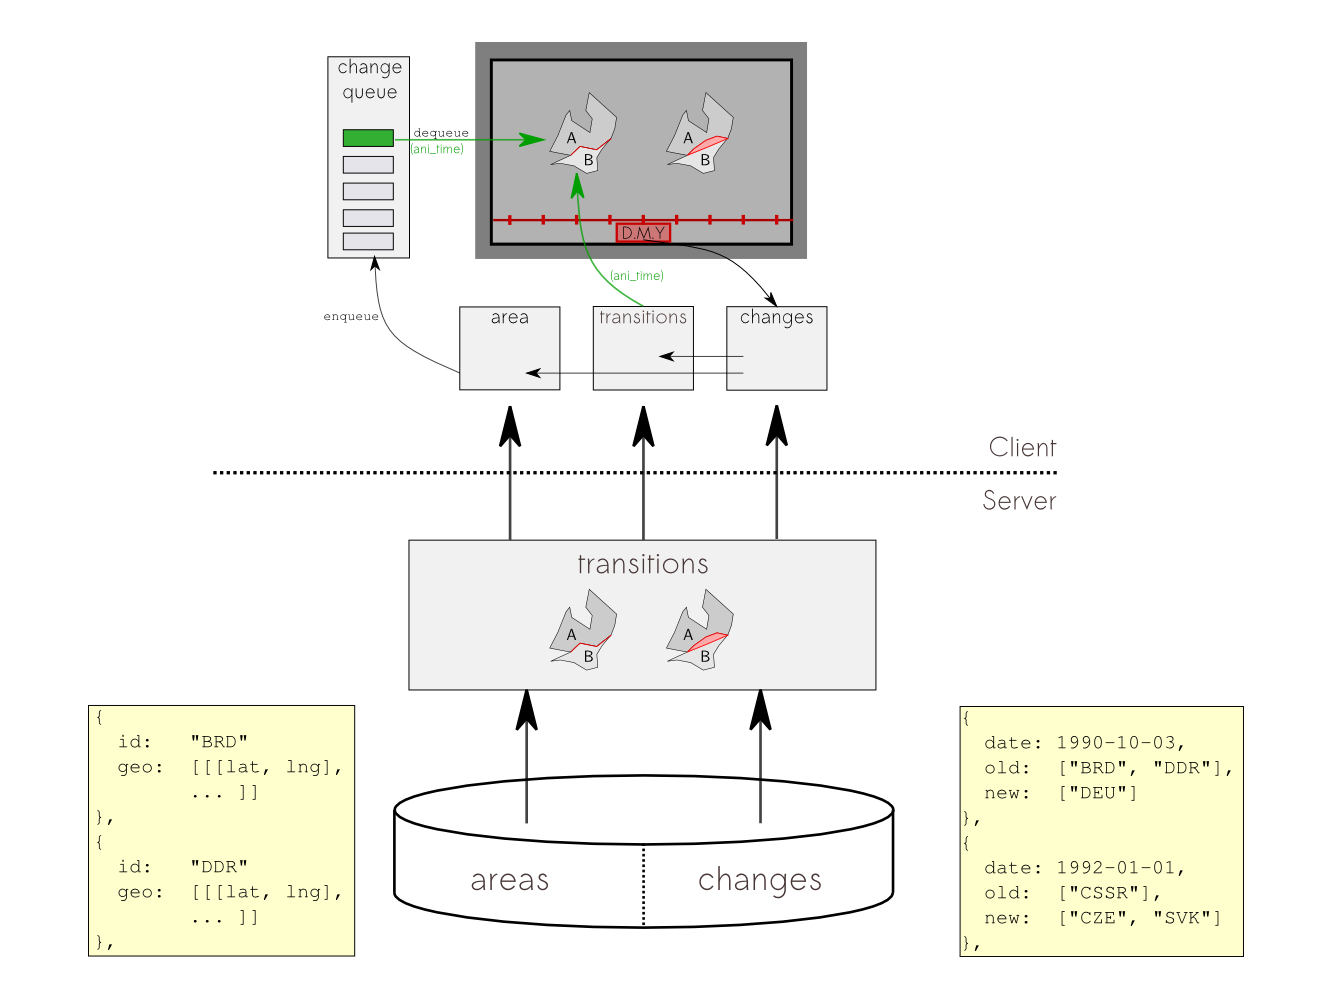
\includegraphics[width=0.9\textwidth]{graphics/historic_countries.png}
  \end{center}
  \caption{Architecture of historic countries on the map}
  \label{fig:historic_changes}
\end{figure}

The countries areas, labels and changes are created, preprocessed with the \textit{Python} script and delivered to the server. The client gets the four \textit{json} files and reads the data from there. When the NowDate on the timeline changes, the timeline sends the old date and the new date to Controller that finds out all the changes happened in time period. From each change the transition areas and borders are faded in on the map and the related old and new areas and labels are enqueued as a change event in a \textbf{change queue}. Every 50 milliseconds the queue is processed: for the first change event it checks if the related transitions are fully faded in. If so, the new areas and labels will be added and the old areas and labels deleted from the map. Finally, the transitions will be faded out again.

For moving the timeline backwards, the mechanism is the same, it is just that old and new areas and labels are swapped, because the historic change happens now the other way.

In order to prevent large amounts of changes on the map if the timeline is moved far, a rule-out mechanism is implemented: There is a list of old and new areas and labels for all historic changes in the period between the old and the new date from the timeline. Areas and labels that would be added in one change but deleted in another change are removed from both lists, because they would not contribute to the visualization. With this mechanism it is possible to move the timeline at a high speed there and back and always get a consistent update on the map without irritating the user.

\subsubsection{Styling the Countries} % (fold)
\label{ssub:styling_the_countries}

% subsubsection styling_the_countries (end)

